\clearpage

\section {Neutrino oscillation fitting}
\label{sec:oscfit}

%--------------------------------------------------------------------------------------------------------------------
\subsection {Fit method}
\label{sec:oscfit_method}

One of the motivations for this analysis is to determine whether the oscillation parameters for $\bar{\nu}_{\mu}$ disappearance are different 
from those for $\nu_{\mu}$ disappearance. For this reason, two separate sets of oscillation parameters are used. The first set consists of  
$\sin^{2}\overline{\theta}_{23}$, $\sin^{2}\overline{\theta}_{12}$, $\sin^{2}\overline{\theta}_{13}$, $|\overline{\Delta m}^{2}_{32}|$ 
(normal hierarchy) or $|\overline{\Delta m}^{2}_{31}|$ (inverted hierarchy), 
$\overline{\Delta m}^{2}_{21}$ and $\delta_{CP}$, and these parameters are 
applied to the $\bar{\nu}_{\mu}$, $\bar{\nu}_{e}$ and oscillated $\bar{\nu}_{e}$ interaction modes. The other set of oscillation parameters is 
$\sin^{2}\theta_{23}$, $\sin^{2}\theta_{12}$, $\sin^{2}\theta_{13}$, $|\Delta m^{2}_{32}|$ 
(normal hierarchy) or $|\Delta m^{2}_{31}|$ (inverted hierarchy),
$\Delta m^{2}_{21}$ and $\delta_{CP}$, and they are applied to the $\nu_{\mu}$, $\nu_{e}$ and oscillated $\nu_{e}$
interaction modes. All these parameters are fixed in the fits of the Super K data except $\sin^{2}\overline{\theta}_{23}$ 
and $|\overline{\Delta m}^{2}_{32}|$ 
(normal hierarchy) or $|\overline{\Delta m}^{2}_{31}|$ (inverted hierarchy); 
these fixed values are the T2K+reactor best-fit values and are shown in Tab.~\ref{tab:osc_params_fixed_values_reactor}.

\begin{table}
\centering
 \begin{tabular}{| c | c | c |}
% \hline
% Parameter(s)                                               			&     Treatment              &           Nominal value (NH)           & Nominal value (IH)      \\
%\hline
%$\sin^{2}\theta_{23}$                                       			&     marginalized         &                \MixingTwoThreeNH       &    \MixingTwoThreeIH  \\
%$\sin^{2}\theta_{13}$  							&     marginalized         &                \MixingOneThreeNH	&      \MixingOneThreeIH	 \\
%$\sin^{2}\theta_{12}$  							&     fixed               	    &             \MixingOneTwoIH             &    \MixingOneTwoIH	 \\
%$|\Delta m^{2}_{32}|$ (NH) / $|\Delta m^{2}_{31}|$ (IH)      &     marginalized          &               \DmsqNH			&      \DmsqIH                        \\
%$\Delta m^{2}_{21}$      							&     fixed                       &             \dmsqIH                          & 	\dmsqIH		\\
%$\delta_{CP}$                                               			&     marginalized           &              \DeltaCPNH			&     \DeltaCPIH              \\
%Mass Hierarchy									&     marginalized	    &           Normal Hierarchy
 \hline
 Parameter(s)                                               			&     Treatment              &           Nominal value 		    \\
\hline
$\sin^{2}\theta_{23}$                                       			&     marginalized         &                \MixingTwoThreeNH        \\
$\sin^{2}\theta_{13}$  							&     marginalized         &                \MixingOneThreeNH	 \\
$\sin^{2}\theta_{12}$  							&     fixed               	    &             \MixingOneTwoIH              \\
$|\Delta m^{2}_{32}|$ (NH) / $|\Delta m^{2}_{31}|$ (IH)      &     marginalized          &               \DmsqNH		          \\
$\Delta m^{2}_{21}$      							&     fixed                       &             \dmsqIH                         	\\
$\delta_{CP}$                                               			&     marginalized           &              \DeltaCPNH		      \\
Mass Hierarchy									&     marginalized	    &            	NH         \\  
\hline
\end{tabular}
\caption{
Treatment of the oscillation parameters in the p-value computation as well as used values for fixed parameters.
The values of the fixed oscillation parameters correspond to the most probable parameters of the bayesian analysis
described in \cite{T2KLongPaper,Mach3JointFitRun14}.
The mass hierarchy is marginalized as well.
}
\label{tab:osc_params_fixed_values_reactor}
\end{table}


The {\em VALOR} disappearance analysis uses a binned likelihood-ratio method.
Measurements of the oscillation parameters $\sin^{2}\overline{\theta}_{23}$ and $|\overline{\Delta m}^{2}_{32}|$ 
or $|\overline{\Delta m}^{2}_{31}|$
are obtained by comparing the observed and predicted SuperK reconstructed energy spectra
for 1-ring $\mu$-like events.

Let $N$ be the number of reconstructed energy bins and
${\bf a}$ be a $1 \times N_{s}$ - dimensional array of systematic (nuisance) 
parameters that affect the SuperK reconstructed energy spectrum prediction (e.g
parameters that control the beam, neutrino interaction simulations and 
the detector response).
Best-fit values are obtained by minimising: 
\begin{equation}
\displaystyle
%\chi^{2} 
-2 \; \textrm{ln} \; \lambda (\sin^{2}\overline{\theta}_{23},|\overline{\Delta m}^{2}_{32}| 
    \; \textrm{or} \; |\overline{\Delta m}^{2}_{31}|
   ; {\bf a}) = 2 \cdot \sum_{i=0}^{N-1} 
   \Big( 
     n^{obs}_{i} \cdot ln(n^{obs}_{i}/n^{exp}_{i}) +
     (n^{exp}_{i}-n^{obs}_{i}) 
   \Big) +
   ({\bf a}-{\bf a_{0}})^{T} \cdot {\bf C}^{-1} \cdot ({\bf a}-{\bf a_{0}})
\label{eq:chisquare}
\end{equation}
where
${\bf a_{0}}$ is an $1 \times N_{s}$ - dimensional array with the default values of 
the systematics parameters, ${\bf a}^{T}$ is the transpose of ${\bf a}$,
${\bf C}$ is the systematic parameter covariance matrix of dimension $N_{s} \times N_{s}$,
$n^{obs}_{i}$ is the observed number of events in the $i^{th}$ bin, and
$n^{exp}_{i} = n^{exp}_{i}(\sin^{2}\overline{\theta}_{23},|\overline{\Delta m}^{2}_{32}| \; \textrm{or} \; |\overline{\Delta m}^{2}_{31}|; {\bf a})$ 
%$n^{exp}_{i} = n^{exp}_{i}(\sin^{2}\overline{\theta}_{23},|\overline{\Delta m}^{2}_{32}|; {\bf a})$ 
is the corresponding expected number of events.

The advantage of the likelihood ratio method over the extended maximum-likelihood method is that,
in the large-sample limit, the quantity 
$-2 \: \textrm{ln} \: \lambda (\sin^{2}\overline{\theta}_{23},|\overline{\Delta m}^{2}_{32}| \; \textrm{or} \; |\overline{\Delta m}^{2}_{31}|; {\bf a})$
%$-2 \: \textrm{ln} \: \lambda (\sin^{2}\overline{\theta}_{23},|\overline{\Delta m}^{2}_{32}|; {\bf a})$
in Eq.\ref{eq:chisquare} has a $\chi^{2}$ distribution and it can therefore be used as a goodness-of-fit test.
In this note,
$-2 \: \textrm{ln} \: \lambda (\sin^{2}\overline{\theta}_{23},|\overline{\Delta m}^{2}_{32}| \; \textrm{or} \; |\overline{\Delta m}^{2}_{31}|; {\bf a})$ and
$\chi^{2}(\sin^{2}\overline{\theta}_{23},|\overline{\Delta m}^{2}_{32}| \; \textrm{or} \; |\overline{\Delta m}^{2}_{31}|; {\bf a})$ are used interchangeably.
%$-2 \: \textrm{ln} \: \lambda (\sin^{2}\overline{\theta}_{23},|\overline{\Delta m}^{2}_{32}|; {\bf a})$ and
%$\chi^{2}(\sin^{2}\overline{\theta}_{23},|\overline{\Delta m}^{2}_{32}|; {\bf a})$ are used interchangeably.


The minimisation is performed with Minuit \cite{Minuit}, using the Migrad method.
If Migrad does not converge, the starting values of the oscillation parameters are re-initialised:
the new initial values are randomly drawn from uniform distributions in the ranges 
$1.5 \times 10^{-3}$ eV$^{2}$/c$^{4}$ $\leq$ $|\overline{\Delta m}^{2}_{32}| \; \textrm{or} \; |\overline{\Delta m}^{2}_{31}|$ $\leq$ $2.0 \times 10^{-2}$  
%$1.5 \times 10^{-3}$ eV$^{2}$/c$^{4}$ $\leq$ $|\overline{\Delta m}^{2}_{32}| \;$ $\leq$ $2.0 \times 10^{-2}$
eV$^{2}$/c$^{4}$ and either 0.35 $\leq$ $\sin^{2}\overline{\theta}_{23}$ $\leq$ 0.50 or 0.53 
$\leq$ $\sin^{2}\overline{\theta}_{23}$ $\leq$ 0.68 (the new initial value of 
$\sin^{2}\overline{\theta}_{23}$ is in the same octant as the previous initial value).  
The fit is retried with the new initial values, and this is repeated up to 10 times.
If the fit still fails to converge after 10 attempts, the Simplex algorithm is used.
For the data and Asimov dataset analysis described in this document, this fallback was never triggered.
The search for the minimum value of 
$-2 \: \textrm{ln} \: \lambda(\sin^{2}\overline{\theta}_{23},|\overline{\Delta m}^ {2}_{32}| \; \textrm{or} \; |\overline{\Delta m}^{2}_{31}|; {\bf a})$ (see Eq.~\ref{eq:chisquare}) 
%$-2 \: \textrm{ln} \: \lambda(\sin^{2}\overline{\theta}_{23},|\overline{\Delta m}^ {2}_{32}|; {\bf a})$ (see Eq.~\ref{eq:chisquare})
is performed in the range 
$0 \leq$ $\sin^{2}\overline{\theta}_{23}$ $\leq 1$ and
$1 \times 10^{-3}$ eV$^{2}$/c$^{4}$ $\leq$ $|\overline{\Delta m}^{2}_{32}| \; \textrm{or} \; |\overline{\Delta m}^{2}_{31}|$ $\leq 2 \times 10^{-2}$ eV$^{2}$/c$^{4}$. 
%$1 \times 10^{-3}$ eV$^{2}$/c$^{4}$ $\leq$ $|\overline{\Delta m}^{2}_{32}| \; $ $\leq 2 \times 10^{-2}$ eV$^{2}$/c$^{4}$.
After a successful fit, The Hesse algorithm is called to improve Minuit's estimates of the errors on the fitted parameters.

Each fit is repeated twice: in the first fit, the initial values are $|\overline{\Delta m}^{2}_{32}|$ 
or $|\overline{\Delta m}^{2}_{31}|$ 
= 2.4 $\times$ 10$^{-3}$ 
eV$^{2}$/c$^{4}$ and $\sin^{2}\overline{\theta}_{23} = 0.6$, while the second fit uses as initial values the best fit of $|\overline{\Delta m}^{2}_{32}|$ 
or $|\overline{\Delta m}^{2}_{31}|$ 
and the mirror point in the other octant of the best fit of $\sin^{2}\overline{\theta}_{23}$ from the first fit. 

All the systematic parameters are allowed to float in the fit, and are restricted to the range [-3$\sigma_{s}$, +3$\sigma_{s}$]
where $\sigma_{s}$ is the one standard deviation error assigned to each systematic parameter.

Values of systematic parameters that give a negative predicted number of events in any reconstructed energy bin in any interaction 
mode are not allowed. If a systematic throw gives a negative number of events, that toy experiment is rejected.

%--------------------------------------------------------------------------------------------------------------------                                                                                    

\subsection {Goodness-of-fit tests}
\label{sec:gof_test}

The goodness-of-fit tests are done by minimising the expression in equation \ref{eq:chisquare}. In this analysis, the same 
coarse binning is used for these tests as in our neutrino-mode $\nu_{\mu}$-disappearance analyses 
\cite{OurRun123DisappAnalysis3Flavour}, \cite{OurRun1234aDisappAnalysis3Flavour} and \cite{OurRun1234DisappAnalysis3Flavour}. 
The choice of this binning followed a decision by the oscillation analysis group that p-values should be calculated using the rate 
and the reconstructed energy distribution, and that a very coarse binning scheme should be used to ensure that there are 
sufficient numbers of events in each bin; this scheme has 5 bins from 0-0.4, 0.4-0.7, 0.7-1.0, 1.0-2.0 and 2.0-30.0 GeV.
The Asimov spectrum using this binning can be seen in figure~\ref{fig:1Rmu_spectrum_gof}.
1000 toy experiments are generated for each mass hierarchy, and both systematic variations and statistical 
fluctuations are applied to them. All \NSyst{} systematic parameters are included in the fits of those datasets. 
\begin{figure}
\center
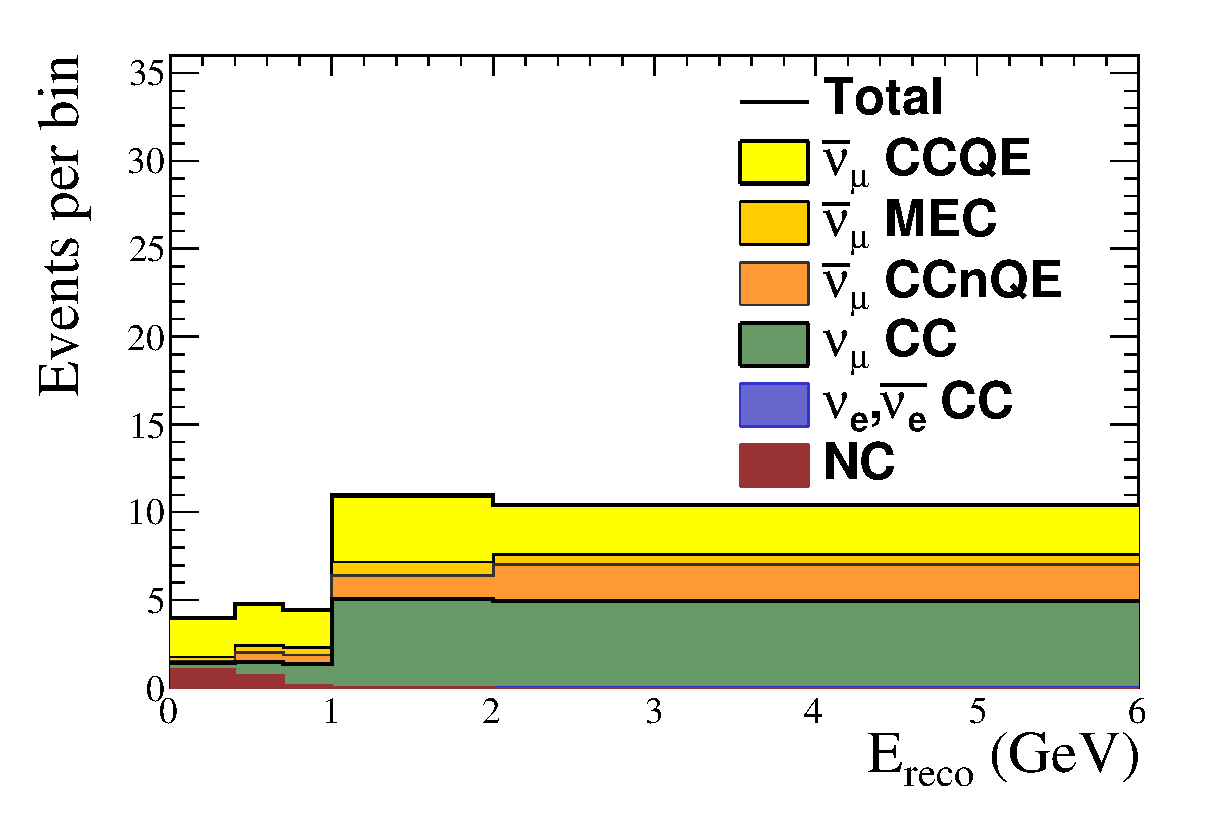
\includegraphics[width=0.8\linewidth]{./images/spectrum_predictions/sk_ereco_spectrum_RHC1Rmu_spectrum_reactor_postfit_gof_0.527000_0.002510_grouped.eps}
\caption {
Predicted reconstructed-energy spectrum of 1 $\mu$-like ring events,
for the postfit Asimov dataset, using the Goodness-of-Fit binning,
for an exposure of \TotalPot POT in antineutrino beam mode.
Event counts are shown as total per bin, without accounting for bin width.
Oscillations are applied at the values from table~\ref{tab:osc_params_fixed_values_reactor}.
Note that the highest bin here, from 2.0 GeV onwards contains all events at with energies greater than 2.0 GeV.
}
\label{fig:1Rmu_spectrum_gof}
\end{figure}

%--------------------------------------------------------------------------------------------------------------------                                                                                    

\subsection {Construction of confidence regions}
\label{sec:contour_construction}

In this analysis, uncertainties in the jointly measured parameters are quoted using
%~ both
the constant-$\Delta\chi^{2}$ \cite{PDG2012} (pp. 390-401).
%~ and the Feldman-Cousins \cite{FeldmanCousins} methods.
%~ A definite recommendation was made in favour of the Feldman and Cousins method
%~ for constructing confidence regions by the T2K $\nu_{\mu}$ contour committee \cite{T2KNuMuContourCom}.
%~ The work of Feldman and Cousins
%~ uses the freedom which is inherent in the Neyman construction of confidence regions
%~ to address cases
%~ (in particular, cases with
%~ Poisson processes with background and Gaussian errors near a physical boundary)
%~ where the classical construction of confidence regions produces overcoverage, undercoverage, or
%~ in extreme cases, an empty region.

%~ The two methods have been described in detail in past T2K technical notes and presentations.
%~ For completeness, we summarise both of these methods here
%~ and provide definite statements on the exact methodology used for incorporating systematic errors.

%~ The methods differ in the calculation of the critical values of $\Delta{\chi^{2}}$, which are used to identify the areas 
%~ of the parameter space to be included in the allowed region for a given confidence level. The constant-$\Delta\chi^{2}$ 
%~ method is a fully frequentist treatment using the Gaussian approximation.
One finds the best-fit point and calculates the confidence contours as lines of \emph{constant} $\Delta{\chi^{2}}$
from this point\footnote{
For 1 fit parameter, the critical values of $\Delta{\chi^{2}}$ used are
1.00 (68\% CL), 2.71 (90\% CL), 3.84 (95\% CL), 6.63 (99\% CL).
For 2 parameters fitted simultaneously, the critical values of $\Delta{\chi^{2}}$ used are
2.30 (68\% CL), 4.61 (90\% CL), 5.99 (95\% CL), 9.21 (99\% CL).
}.

%~ The method of Feldman and Cousins method finds the critical values of $\Delta{\chi^{2}}$ as follows: many toy MC experiment 
%~ fits are performed for each point of the ($\sin^{2}\overline{\theta}_{23}$, $|\overline{\Delta m}^{2}_{32}|$ or $|\overline{\Delta m}^{2}_{31}|$) 2-dimensional grid.
%~ The value of $\Delta\chi^{2}_{MC}$ for each toy MC experiment is calculated as
%~ \begin{equation}
%~ \displaystyle
%~ \Delta \chi^{2}_{MC} = \chi^{2} \textrm{(MC, true)} - \chi^{2} \textrm{(MC, best fit)}
%~ \label{eq:deltachi2mc}
%~ \end{equation}
%~ where
%~ ``true'' means that the $\chi^{2}$ was computed using the true values of the oscillation parameters at that grid point, and
%~ ``best-fit'' means that the $\chi^{2}$ was computed using the actual best-fit values for that MC experiment.
%~ The $\chi^{2}$ values are calculated using Eq.~\ref{eq:chisquare}.
%~ For each grid point, the critical value of $\Delta\chi^{2}$ ($\Delta\chi^{2}_{critical}$)
%~ is found such that $\alpha$ of the toy MC experiments have $\Delta\chi^{2}_{MC}$ $<$ $\Delta\chi^{2}_{critical}$,
%~ where $\alpha$ is the desired confidence level.
%The Feldman and Cousins confidence regions for a fit to an actual dataset are drawn such that grid points 
%with $\Delta\chi^{2}_{data}$ $<$ $\Delta\chi^{2}_{critical}$ are included within the contour, 
%where $\Delta\chi^{2}_{data}$ is given by
%\begin{equation}
%\displaystyle
%\Delta \chi^{2}_{data} = \chi^{2} \textrm{(true)} - \chi^{2} \textrm{(data, best fit)}
%\label{qe:fccontour}
%\end{equation} 
%~ The principal difference between the Feldman and Cousins and the constant $\Delta\chi^{2}$ methods is that the former determines 
%~ the value of $\Delta\chi^{2}_{critical}$ individually for each grid point, whereas the latter uses the same value 
%~ for all grid points.

The procedure for constructing the $\Delta\chi^{2}(\sin^{2}\overline{\theta}_{23},|\overline{\Delta m}^{2}_{32}| \; \textrm{or} \; |\overline{\Delta m}^{2}_{31}|)$
surface itself from the T2K Run 5+6 data is 
as follows: 
%~ common to both methods:
assuming that N nuisance parameters are allowed to float in the oscillation fit,
the values of $\chi^{2}(\sin^{2}\overline{\theta}_{23},|\overline{\Delta m}^{2}_{32}| \; \textrm{or} \; |\overline{\Delta m}^{2}_{31}|; {\bf a})$
are calculated via a fit at \emph{each} point of the ($\sin^{2}\overline{\theta}_{23}$, $|\overline{\Delta m}^{2}_{32}|$ or $|\overline{\Delta m}^{2}_{31}|$)
2-dimensional grid, where only the nuisance parameters are allowed to float
and $\sin^{2}\overline{\theta}_{23}$ and $|\overline{\Delta m}^{2}_{32}|$ or $|\overline{\Delta m}^{2}_{31}|$ are fixed to the true values for the given grid point.
The following grid spacing is used
%~ in all confidence region construction methods
: $\delta{\sin^{2}\overline{\theta}_{23}}$ = 5$\times$10$^{-3}$ and
$\delta |\overline{\Delta m}^{2}_{32}| \; \textrm{or} \; \delta |\overline{\Delta m}^{2}_{31}|$ = 5$\times$10$^{-5}$ eV$^{2}$/c$^{4}$.

The allowed region in the 2D oscillation parameter space is then given by
\begin{equation}
\displaystyle
\Delta\chi^{2}(\sin^{2}\overline{\theta}_{23},|\overline{\Delta m}^{2}_{32}| \; \textrm{or} \; |\overline{\Delta m}^{2}_{31}|) =
\chi^{2}(\sin^{2}\overline{\theta}_{23},|\overline{\Delta m}^{2}_{32}| \; \textrm{or} \; |\overline{\Delta m}^{2}_{31}|; {\bf a}) - \chi_{min}^{2} < \Delta{\chi^{2}}_{critical}
\label{eq:chiconfregion}
\end{equation}
where $\chi_{min}^{2}$ is the minimum value of $\chi^{2}(\sin^{2}\overline{\theta}_{23},|\overline{\Delta m}^{2}_{32}| \; \textrm{or} \; |\overline{\Delta m}^{2}_{31}|; {\bf a})$
from the fit of the T2K Run 5+6 data over the oscillation parameter space considered.
%~ 
%~ The Feldman and Cousins method does not specify how systematics are to be included 
%~ in the confidence region construction and different choices exist. 
%~ To construct a 2-dimensional ($\sin^{2}\overline{\theta}_{23}$, $|\overline{\Delta m}^{2}_{32}|$ or $|\overline{\Delta m}^{2}_{31}|$) confidence region, 
%~ where N systematic parameters are included in the p.d.f. and all of these N systematics are allowed to float in the fit,
%~ this analysis uses the following methodology: 
%~ the value of $\Delta\chi^{2}_{critical}$ at each true ($\sin^{2}\overline{\theta}_{23}$, $|\overline{\Delta m}^{2}_{32}|$ or $|\overline{\Delta m}^{2}_{31}|$) grid point 
%~ is calculated from an ensemble of toy MC experiments,
%~ each one of which is generated with the true oscillation parameters of that point and with all N systematics randomised.
%~ For each toy MC experiment, both $\sin^{2}\overline{\theta}_{23}$, $|\overline{\Delta m}^{2}_{32}|$ or $|\overline{\Delta m}^{2}_{31}|$ and all N nuisance parameters are fitted
%~ simultaneously to obtain the value of $\chi^{2} \textrm{(MC, best fit)}$ used in Eq.~\ref{eq:deltachi2mc}.
%~ A separate fit, with $\sin^{2}\overline{\theta}_{23}$ and $|\overline{\Delta m}^{2}_{32}|$ or $|\overline{\Delta m}^{2}_{31}|$ fixed to their true values
%~ and with all N nuisance parameters allowed to float, is performed to obtain the value of 
%~ $\chi^{2} \textrm{(MC, true)}$ (i.e.\ $\chi^{2}$ is \emph{independently} minimised, for \emph{each} toy MC experiment, with 
%~ respect to the nuisance parameters).  

